\chapter{The LHC}
\label{ch:lhc}
%P1, what is the LHC?
\par The Large Hadron Collider, abbreviated as LHC, is the most powerful proton-proton collider, located at CERN, Geneva, Switzerland. The LHC is installed in a 26.7 km tunnel that was built for last generation lepton collider between 1984 and 1989. The LHC tunnel, which is located from 45m to 170m below the surface, is composed of 8 straight sections and 8 arcs. Therefore, the LHC can be viewed as 8 octants. Each octant has an access point, which includes an elevator from surface to underground. Half of the LHC points are hosting the detector systems currently: ATLAS\cite{Aad:2008zzm} at Point 1, ALICE\cite{Aamodt:2008zz} at Point 2, CMS\cite{Chatrchyan:2008aa} at Point 5 and LHCb\cite{Alves:2008zz} at Point 8. The other 4 points are designed for LHC operation purposes.

%P2, the LHC, history, and future
\par Rome wasn's built in one day, neither was the LHC. The LHC was built on the infrastructure of the previous generation of colliders located at CERN. The LHC is the current frontier of the evolution chain shown in Fig~\ref{fig:c3cernaccs}: from Proton Synchrotron (1954)\cite{Gilardoni:2011za}, Super Proton Synchrotron (1976)\cite{Doble:2017syb}, Large Electron-Positron Collider (1984)\cite{LepInjectorStudy:1983aa}\cite{LepInjectorStudy:1983ab}, to Large Hadron Collider (2008)\cite{Bruning:2004ej}\cite{Buning:2004wk}. Both infrastructure and technology are utilized in an economic manner to support the most powerful collider in the world, the LHC. The proton beam can be accelerated at 7 TeV by the current LHC setup. Although the LHC has reached the frontier of the high energy of human experiment, it is not the end of the CERN collider evolution chain. Both the LHC upgrade plan\cite{ApollinariG.:2017ojx} and next generation collider design\cite{Benedikt:2018csr} have been proposed to sustain the prosperity of the CERN collider family.

\begin{figure}[htbp]
    \centering
    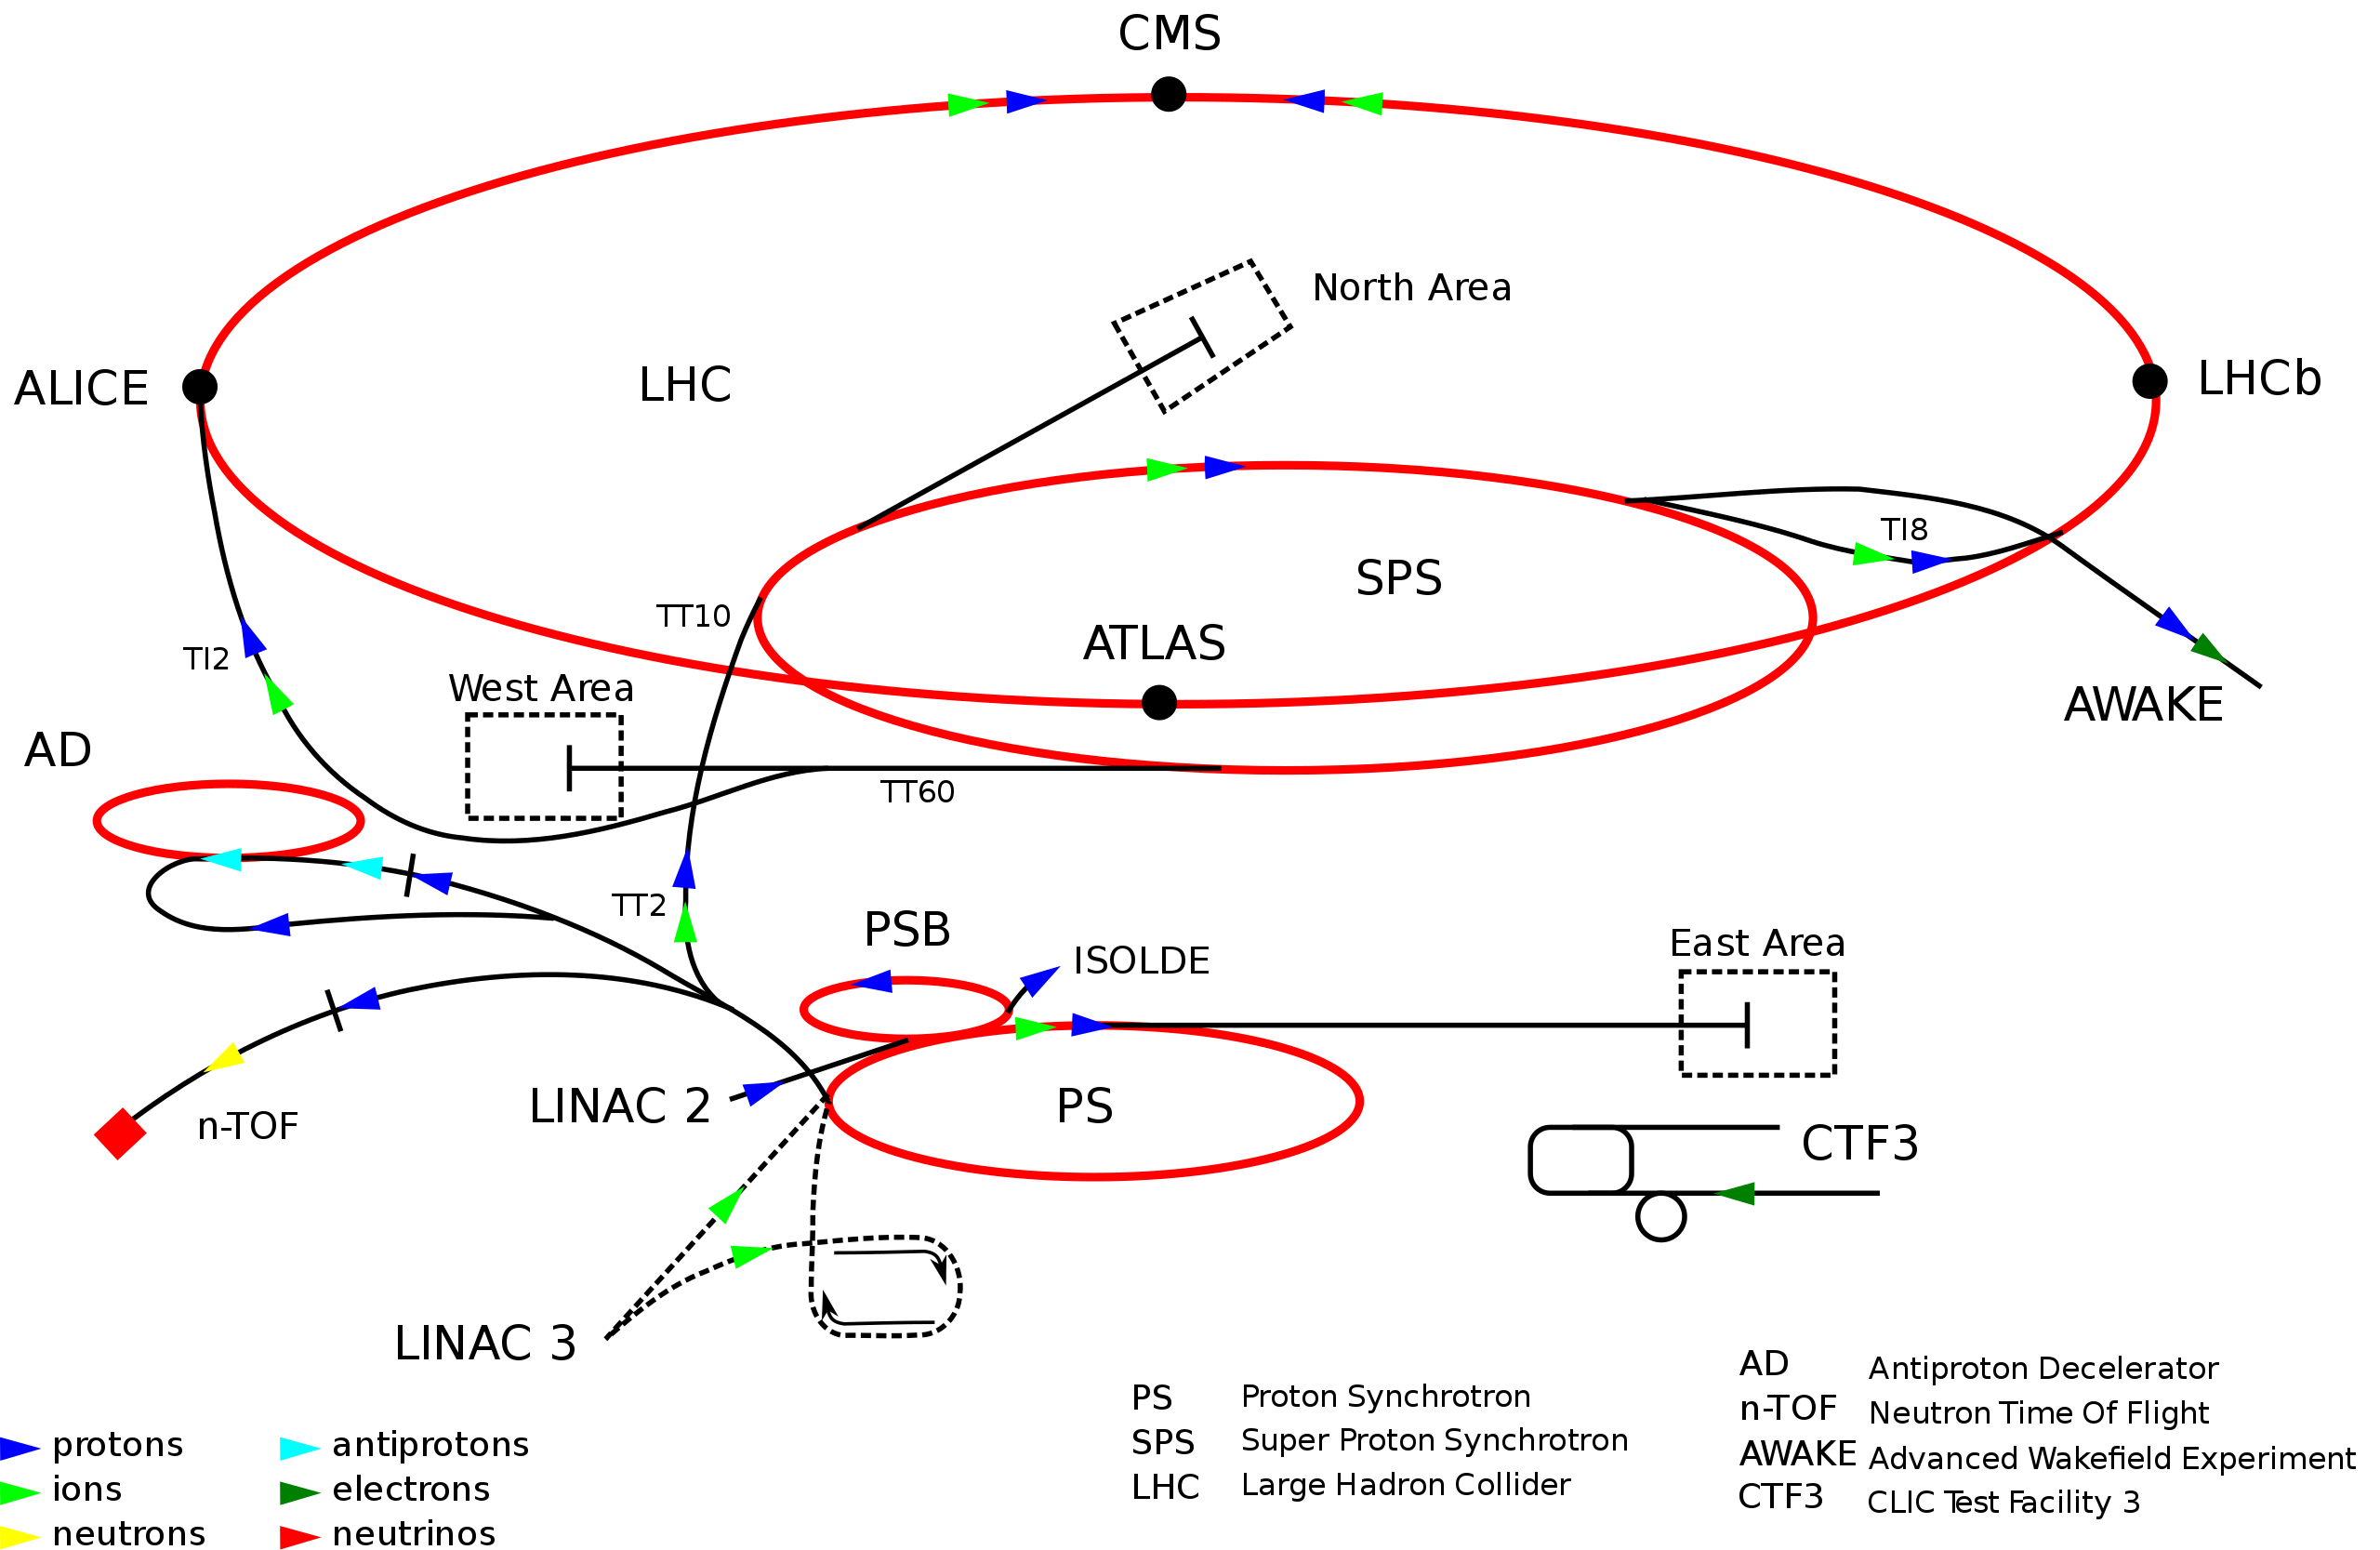
\includegraphics[width=0.8\textwidth]{chapters/c3/figures/cern-accelerator-complex.png}
    \caption{The LHC full injection chain.}
    \label{fig:c3cernaccs}
\end{figure}

\section{The LHC performance}
\label{sec:lhcs1}
%P1, the LHC performance and collision data collection: how many data do we take at what energy?
\par The aim of the LHC is to provide a stable, large amount of proton-proton collision events at the high energy frontier. Therefore, the LHC performance can be viewed as two parameters: the center-of-mass energy and integrated luminosity.

\subsection{Beam energy}
%P1, what energy? how to achieve
\par The center-of-mass energy is defined as the proton pair kinetic energy in the center-of-mass frame. Currently, the LHC is running at 13 TeV center-of-mass energy, with 6.5 TeV for each beam. Protons are accelerated and bended by electric field strips and 1232 superconducting dipole magnets around the LHC ring. Higher beam energy requires a stronger magnetic field, which requires to a higher electric current flowing in the magnets' superconducting coils.

\subsection{Luminosity}
%P1, how many data, lumi, definition, equation
\par The integrated luminosity, defined as the number of collision events produced by the LHC inside the particle detector, reflects the number of collisions delivered by the LHC. The integrated luminosity is determined by the LHC instantaneous luminosity, the beam cross-section and total LHC collision time.

\par The LHC luminosity can be calculated by Eq~\ref{eq:c3lumi}, where $N_{b}$ is the number of protons per bunch, $n_{b}$ is number of filled bunches per beam, $f_{r}$ is the frequency of the beam circling the ring, $\gamma_{r}$ is the relativistic gamma factor of the protons, $\epsilon_{n}$ is the normalized transverse beam emittance, $\beta^{*}$ is the measure of beam width in the longitudinal direction, $F$ is a geometric factor which accounts for the non-zero crossing angle between two beams:

\begin{equation}
  L = \frac{N_{b}^{2}n_{b}f_{r}\gamma_{r}4\pi\epsilon_{n}\beta^{*}}{F},
  \label{eq:c3lumi}
\end{equation}

\par The LHC can be running on different luminosity modes, while the detector system needs to be tuned to adapt the various LHC luminosity. The last parameter, total LHC collision time, is an operational parameter that depends on the collider and detector operation teams. The LHC delivered around 156 $fb^{-1}$ data during the Run 2 period as shown in Fig~\ref{fig:lumi0}.
\begin{figure}[htbp]
    \centering
    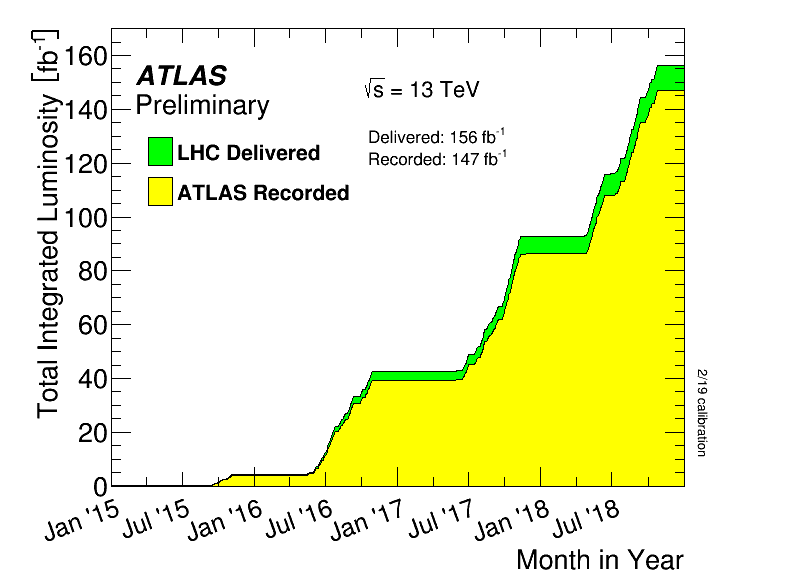
\includegraphics[width=0.8\textwidth]{chapters/c4/figures/intlumivstimeRun2}
    \caption{Cumulative luminosity versus time delivered to ATLAS (green), recorded by ATLAS (yellow) during stable beams for pp collisions at 13 TeV centre-of-mass energy in 2015-2018.}
    \label{fig:lumi}
\end{figure}

\section{The LHC operation}
\label{sec:lhcs1}
%P1, the LHC operation and detector operation, why beam mode
%\par The LHC is a collider with extremely complicated hardware and software design. Fortunately, the LHC team provide a concise operational guide to make physicists understand the LHC running status, which is very helpful during the detector operation. The LHC running status is very important for the detector operation, for example, the detector operator needs to monitor the LHC status and prepare detector configuration, like trigger menu, according to the beam injection notification. Normally, detector operators arrange the detector related activities according to the beam mode.

%P2, beam mode, table
\par The LHC beam modes are explained in Table~\ref{tab:c3lhcbeammode}. The beam modes describe the status of the beam related activities in the LHC. A successful beam injection starts with BEAM SETUP mode, which means beam circulating inside the Super Proton Synchrotron and waiting to be injected into the LHC. Then, a probe beam will be injected into the LHC ring as a trial, which is INJECTION PROBE BEAM mode. After that, INJECTION SETUP BEAM comes to measure the beam properties. After all the previous preparation, the physics injection finally comes into the LHC, which is called INJECTION PHYSICS BEAM. Normally, the detector operators need to get the detector system prepared when an injection physics beam happens. Then, the proton beam will be accelerated in the LHC with the PRERAMP and RAMP mode. The LHC system operators work on final machine adjustment at the FLAT TOP mode, and the beam impact parameter is reduced during the SQUEEZE mode. Finally, the beam is aligned in the ADJUST mode and STABLE BEAM mode will happen. Only the data taken during the STABLE BEAM mode will be used in physics analysis.

\begin{table}[htbp]
\fontsize{10 pt}{1.2 em}
\selectfont
\begin{centering}
\caption{\label{tab:c3lhcbeammode} LHC beam modes.}
\hspace*{-4ex}
\begin{tabular}{|c|c|c|}
\hline
 Mode Name &  Description \\
\hline
 SETUP & \specialcell{Beam in transfer line, but not in the ring} \\
\hline
 ABORT & \specialcell{Recovery mode following beam drop} \\
\hline
 INJECTION PROBE BEAM & \specialcell{Ring is injected with test beam for safe circulating} \\
\hline
 INJECTION SETUP BEAM & \specialcell{Beam measurement going on after probe beam\\ but before injection physics beam} \\
\hline
 INJECTION PHYSICS BEAM & \specialcell{Beam for physics is injected in the ring} \\
\hline
 PRERAMP & \specialcell{Injection done, prepare for ramp} \\
\hline
 RAMP & \specialcell{Ramp up the beam energy} \\
\hline
 FLAT TOP & \specialcell{Ramp done, pre-squeeze checks} \\
\hline
 SQUEEZE & \specialcell{Squeezing the beam size} \\
\hline
 ADJUST & \specialcell{Preparing for collision or after collision} \\
\hline
 STABLE BEAMS & \specialcell{Stable collision, detector should taking data} \\
\hline
 UNSTABLE BEAMS & \specialcell{Unstable beam because of sudden beam degradation} \\
\hline
 BEAM DUMP WARNING & \specialcell{Beam dump warning in case of emergency beam dump} \\
\hline
 BEAM DUMP & \specialcell{End of physics collision} \\
\hline
 RAMP DOWN & \specialcell{Ramp down beam energy after programmed dump} \\
\hline
 CYCLING & \specialcell{Pre-cycle before injection\\ following access, recovery, etc} \\
\hline
 NO BEAM  & \specialcell{No beams exist} \\
\hline
\end{tabular}
\par\end{centering}
\end{table}
